% !TEX root = RKWard_paper.tex
\section{Using RKWard - an example RKWard session}
\label{sec:using_RKWard}
This section describes an example RKWard session, in order to give an idea
of what working with RKWard is like in practice.
The session is organized along the routine tasks of importing,
analyzing, and visualizing data. In this example, it is assumed that an experimental
treatment was given to 20 test subjects, and the objective is to compare the responses
before and after the treatment. 

\subsection{Importing data}
\label{sec:importing_data}
Suppose that the data was saved as or exported to CSV format, for example, from a
spreadsheet application. RKWard's import plugin can
comfortably read it into a new \proglang{R} object.
The import dialog (``File$\rightarrow$Import$\rightarrow$Import
format$\rightarrow$Import Text / CSV data'') assists in reading the
data by a common point \& click interface (Figure~\ref{fig:import_data}A). In this
example, ``comma'' and ``period'' were chosen via ``Quick mode'' as the field
separator and decimal point characters respectively.

The generated \proglang{R} code can be revealed by clicking on the ``Code'' button:

\code{read.csv(file=`/media/software/experiment.txt', 
na.strings = `NA', nrows = -1, skip = 0,
check.names = TRUE, strip.white = FALSE, blank.lines.skip = TRUE)\\}


Checking the ``Edit Object'' box automatically opens a data editor tab
showing the imported data (Figure~\ref{fig:import_data}B).

\begin{figure}[htp]
 \centering
 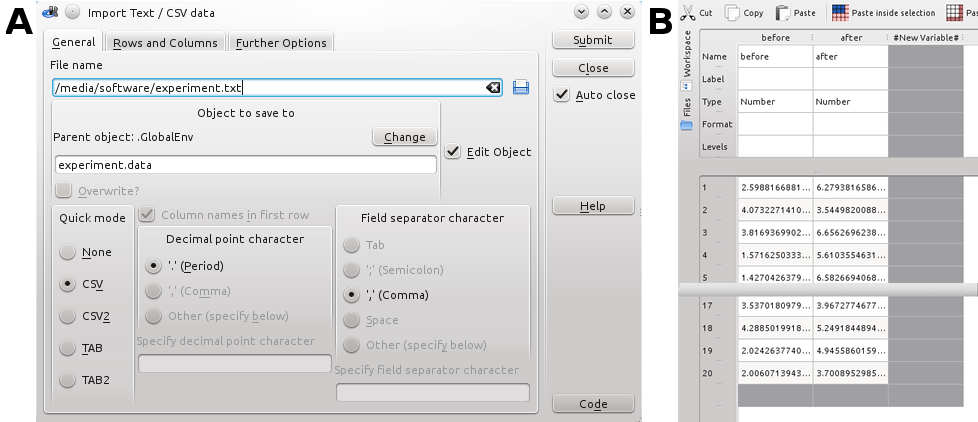
\includegraphics[width=15.5cm]{../figures/import_data.png}
 \caption{A) CSV import dialog. Useful defaults for a variety of common text separated value formats can
  be set using the ``Quick Mode'' selector on the left. Beyond that, many options can be customized. B) Data editor. The imported CSV
  data from experiment.txt are presented (data visually trimmed).}
 \label{fig:import_data}
\end{figure}

\subsection{Conducting a Student's t-test}
\label{sec:conducting_ttest}
To test the hypothesis that the given treatment significantly increased the response, a Student's
t-test for a paired sample is conducted using the 
``Analysis$\rightarrow$Means$\rightarrow$t-Tests$\rightarrow$Two variable t-test'' plugin. 
In the object browser on the left side, the two variables from the expanded
\proglang{R} object containing the table of imported data 
are selected (Figure~\ref{fig:t_test}A). 
Pressing the ``Submit'' button opens the output document tab
showing the results (Figure~\ref{fig:t_test}B).

\begin{figure}[htp]
 \centering
 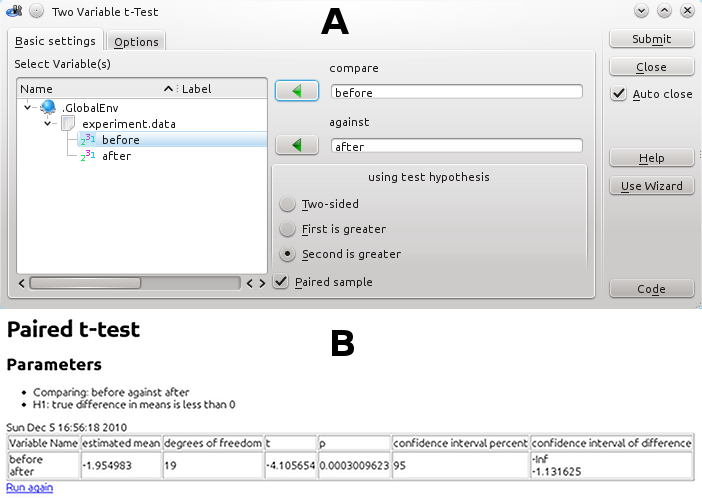
\includegraphics[width=15.5cm]{../figures/t-test.png}
 \caption{A) Student's t-test dialog for two variables. B) Test results in tabular \proglang{HTML} format. 
Besides the result, information such as the date of analysis and the relevant test parameters are also reported.}
 \label{fig:t_test}
\end{figure}



\subsection{Creating a plot}
\label{sec:create_plot}
To visualize the data, ``Boxplot'' is chosen from the ``Plots'' menu
and the two variables, corresponding to the t-test above, are selected.
The dialog allows to define custom variable labels (Figure~\ref{fig:boxplot1}).
Checking the ``Preview'' box opens a graphics window showing the boxplot as
it is configured, and updates the window in real time on any changes to plot parameters. From
that window, the plot can then be exported to several image formats (Figure~\ref{fig:boxplot2}).

\begin{figure}[htp]
 \centering
 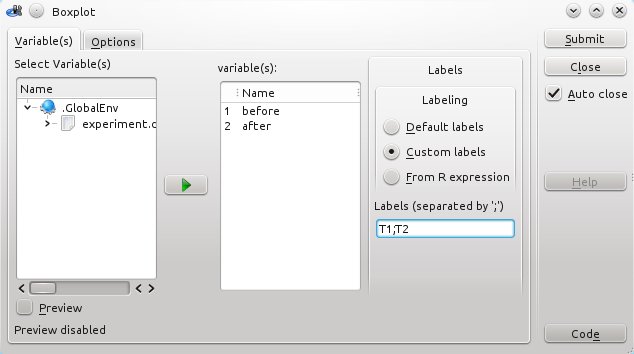
\includegraphics[width=15.5cm]{../figures/boxplot1.png}
 \caption{Boxplot dialog. The first tab (``Variables'') is used to select the variables for analysis. It is possible to
  combine any data present in \code{.GlobalEnv}. The second tab ``Options'' allows further adjustments (e.\,g., the addition of mean and standard deviation) to the plot (not shown).}
 \label{fig:boxplot1}
\end{figure}


\begin{figure}[htp]
 \centering
 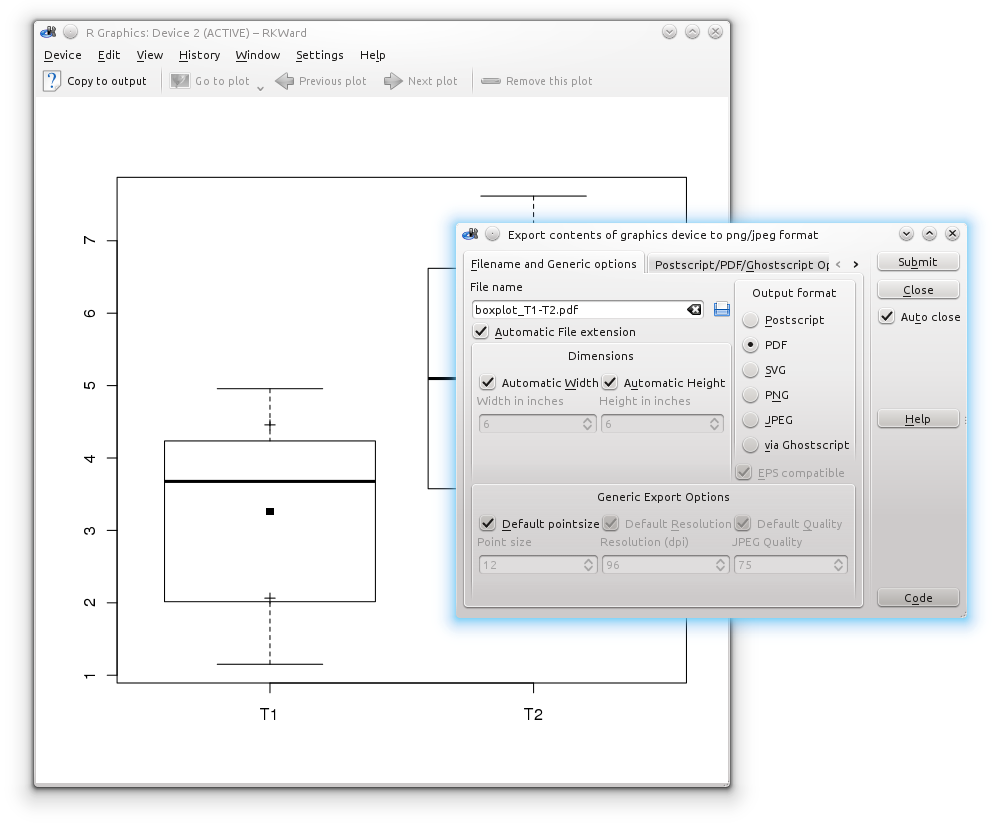
\includegraphics[width=15.5cm]{../figures/boxplot2.png}
 \caption{Plotted data and plot export dialog. The export dialog (``Device$\rightarrow$Export'') provides numerous 
  options like resolution and size for different vector formats (e.\,g., SVG, PDF) and 
  pixel formats (e.\,g., PNG, JPEG). (Note: For the shown figure, the optional  
  mean ($\blacksquare$) and standard deviation ($+$) parameters were selected in the boxplot plugin.)}
 \label{fig:boxplot2}
\end{figure}
